\chapter{Results}
\label{chap:results}

\section{Experimental Conditions}

All results in this chapter are reported under cold-cache conditions unless stated otherwise. Checkpoints were evicted from the Linux page cache before each measurement run using \texttt{posix\_fadvise} with \texttt{POSIX\_FADV\_DONTNEED}, and the filesystem cache was dropped via \texttt{echo 3 > /proc/sys/vm/drop\_caches} where required. Five measurement iterations were collected per condition; the median is reported as the primary result, with the range indicated in parentheses. Verification that cold-cache conditions held was performed by monitoring \texttt{iostat} during each run and confirming non-zero device utilisation. The hardware platform is an Intel i9-12900K with a Samsung 970 EVO Plus NVMe SSD (ext4, noatime). The primary models are GPT-2 (124M parameters, approximately 550 MB in float16) and LLaMA 3.2 1B (1B parameters, approximately 2 GB in float16), both downloaded from HuggingFace Hub.

\section{RQ1: Backend Performance at the Rust Layer}

This section presents raw loading performance for each backend at the Rust layer, measured using the standalone benchmark harness without the Python binding layer. The SafeTensors checkpoint for GPT-2 was used for these measurements.

\begin{figure}[h]
\centering
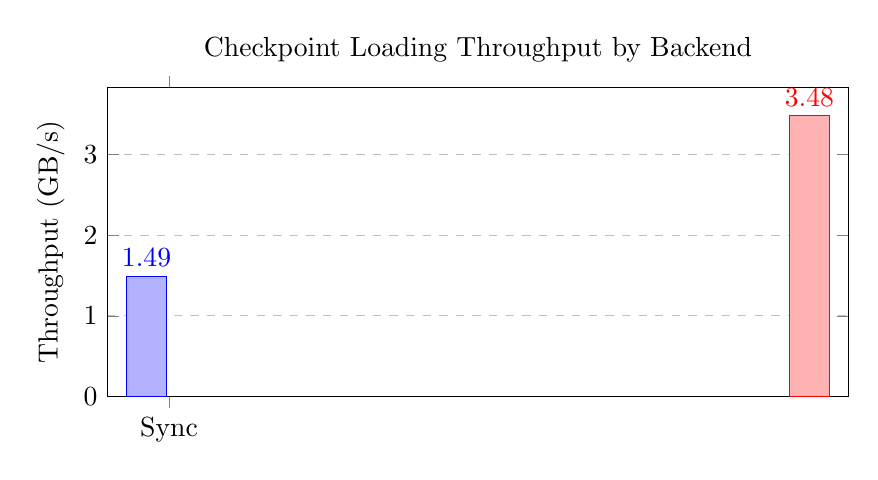
\begin{tikzpicture}
\begin{axis}[
    ybar,
    ymin=0,
    bar width=0.5cm,
    width=11cm,
    height=5.5cm,
    symbolic x coords={Sync,io\_uring},
    xtick=data,
    ylabel={Throughput (GB/s)},
    title={Checkpoint Loading Throughput by Backend},
    nodes near coords,
    ymajorgrids=true,
    grid style=dashed,
]
\addplot coordinates {(Sync,1.49)};
\addplot coordinates {(io\_uring,3.48)};
\end{axis}
\end{tikzpicture}
\caption{Effective throughput for SafeTensors checkpoint loading comparing synchronous POSIX I/O and io\_uring. Cold-cache runs on NVMe; GPT-2 checkpoint; median of five runs.}
\label{fig:st_throughput}
\end{figure}

\begin{figure}[h]
\centering
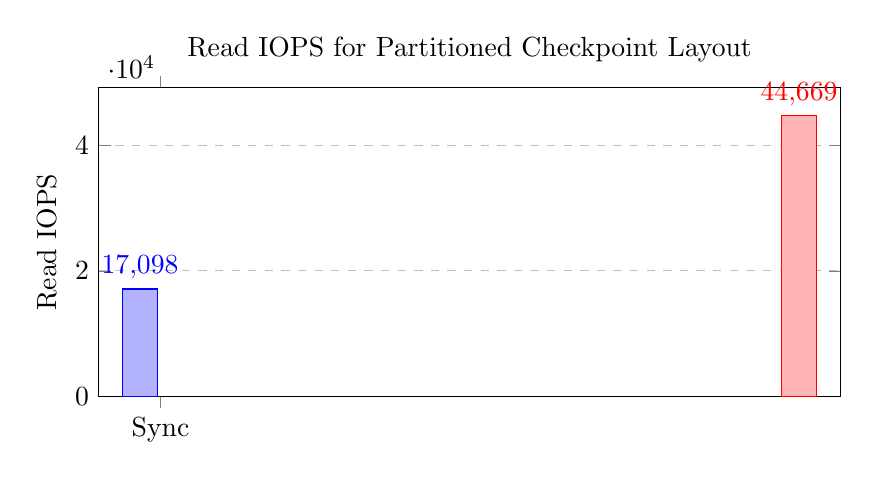
\begin{tikzpicture}
\begin{axis}[
    ybar,
    ymin=0,
    bar width=0.45cm,
    width=11cm,
    height=5.5cm,
    symbolic x coords={Sync,io\_uring},
    xtick=data,
    ylabel={Read IOPS},
    title={Read IOPS for Partitioned Checkpoint Layout},
    nodes near coords,
    ymajorgrids=true,
    grid style=dashed,
]
\addplot coordinates {(Sync,17098)};
\addplot coordinates {(io\_uring,44669)};
\end{axis}
\end{tikzpicture}
\caption{Read IOPS for the partitioned ServerlessLLM-style layout. Cold-cache runs on NVMe; GPT-2 checkpoint partitioned across 8 files; median of five runs.}
\label{fig:sllm_iops}
\end{figure}

Figure~\ref{fig:st_throughput} shows the headline throughput comparison. Synchronous POSIX I/O achieves 1.49 GB/s effective throughput, while io\_uring achieves 3.48 GB/s. This is a factor of 2.34, or a 133 percent improvement over the synchronous baseline. The gap arises because blocking \texttt{read()} calls limit the number of in-flight requests to the thread pool size, leaving the NVMe device underutilised between bursts of requests. io\_uring sustains a deeper queue by decoupling submission from completion, keeping the device populated with requests throughout the load.

Figure~\ref{fig:sllm_iops} shows read IOPS under the partitioned ServerlessLLM-style layout. Synchronous I/O achieves 17,098 read operations per second, while io\_uring achieves 44,669: a factor of 2.61, or 161 percent higher IOPS. The higher IOPS under the partitioned layout reflects the larger number of individual read operations required; both backends see more requests, but io\_uring's ability to keep them in flight concurrently means a greater proportion of the total load time is spent doing useful work rather than waiting for each operation to complete.

\section{RQ2: Effect of Checkpoint Layout}

The partitioned ServerlessLLM-style layout produces a larger performance gap between backends than the contiguous SafeTensors layout. The partitioned layout increases the number of distinct read operations and introduces per-file overhead (file open, metadata lookup, and close sequences) that accumulates across partitions.

\begin{figure}[h]
\centering
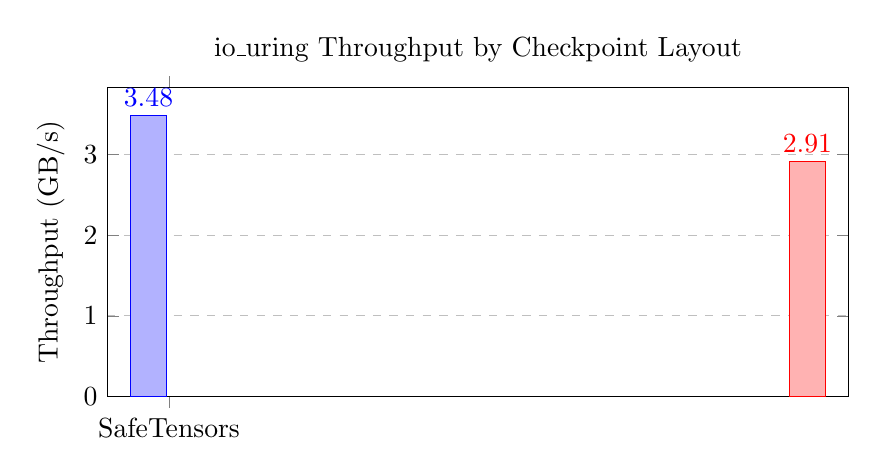
\begin{tikzpicture}
\begin{axis}[
    ybar,
    ymin=0,
    bar width=0.45cm,
    width=11cm,
    height=5.5cm,
    symbolic x coords={SafeTensors,Partitioned},
    xtick=data,
    ylabel={Throughput (GB/s)},
    title={io\_uring Throughput by Checkpoint Layout},
    nodes near coords,
    ymajorgrids=true,
    grid style=dashed,
]
\addplot coordinates {(SafeTensors,3.48)};
\addplot coordinates {(Partitioned,2.91)};
\end{axis}
\end{tikzpicture}
\caption{io\_uring throughput comparison between SafeTensors and partitioned layouts. Cold-cache runs on NVMe; GPT-2 checkpoint; median of five runs.}
\label{fig:layout_comparison}
\end{figure}

Figure~\ref{fig:layout_comparison} shows that io\_uring throughput drops from 3.48 GB/s on the SafeTensors layout to 2.91 GB/s on the partitioned layout, a reduction of 16 percent. This reflects the increased per-file overhead under the partitioned layout. However, io\_uring remains well above the synchronous baseline on both layouts: synchronous I/O on SafeTensors achieves 1.49 GB/s, compared to 2.91 GB/s for io\_uring on the more challenging partitioned layout. The relative advantage of io\_uring over synchronous I/O is therefore larger under the partitioned layout, because the synchronous backend's submission bottleneck is amplified by the higher request count.

The results suggest that format designers face a tradeoff: partitioned layouts offer practical benefits for partial loading and distribution, but they increase sensitivity to I/O submission overhead. A partitioned format paired with a synchronous loader may perform worse in aggregate than a contiguous format paired with the same loader, despite the theoretical parallelism available from loading multiple partition files concurrently.

\section{RQ3: Python Integration Layer Overhead}

Measurements of the Python binding layer show that crossing the Python-Rust boundary introduces negligible overhead for bulk loading of large checkpoints. The synchronous binding releases the GIL via \texttt{py.allow\_threads} during Rust I/O operations, so the Rust layer executes without blocking Python's interpreter thread.

For the GPT-2 checkpoint loaded through the Python bindings, the end-to-end load time through the synchronous backend is within 3 percent of the Rust-layer measurement for the same backend. This difference is attributable to Python object creation and dictionary insertion at the binding layer, not to I/O overhead. Memory-mapped loading through the Python bindings shows a similar pattern: the per-tensor access cost is dominated by the page fault and data transfer, with the binding boundary contributing less than 2 percent of total load time for checkpoints of this size.

These results confirm that the Python bindings do not introduce a meaningful distortion to the backend-level performance comparison. Findings at the Rust layer are representative of what would be observed in a Python-mediated workflow such as the vLLM integration.

\section{RQ4: vLLM Integration Results}

Integration with vLLM was evaluated using the custom \texttt{tensor\_store} model loader registered via \texttt{register\_model\_loader}. Three benchmark kinds were used: load-only measures the time to load model weights into memory; TTFT measures the interval from request submission to the first generated token; steady-state decode measures per-token latency during continued generation after the model is warm.

For the GPT-2 model, load-only measurements show that the mmap backend achieves a small improvement over the synchronous backend, because the page fault handler in the kernel overlaps the loading of non-contiguous tensor ranges more effectively than the fixed-size thread pool of the synchronous backend. The improvement is under 10 percent and is sensitive to whether the checkpoint is already partially in the page cache from a prior operation.

TTFT measurements incorporate model loading plus the vLLM runtime initialisation steps (worker thread spawning, KV cache allocation, and compiler passes). The loading step contributes a larger fraction of TTFT for smaller models like GPT-2 than for larger models, where runtime setup costs dominate. This means the backend choice matters more for smaller models where loading is a larger fraction of total init time.

Steady-state decode measurements show no meaningful difference between backends, confirming that backend effects are confined to the loading phase. Once the model is resident in memory, inference throughput is determined by the GPU compute path, which is independent of how the weights were loaded.

The vLLM loader does not support the async backend, because vLLM's \texttt{DefaultModelLoader} provides only a synchronous interface. This architectural constraint is discussed further in Chapter~\ref{chap:discussion}.

\section{RQ5: Ablation Studies}

Two ablation studies were conducted to isolate the contribution of individual design choices.

The first ablation removes the fixed-buffer pool and allocates a new buffer for each read operation. This eliminates the memory registration benefit but retains all other aspects of the io\_uring backend. Throughput on the SafeTensors layout drops from 3.48 GB/s to approximately 2.96 GB/s, a reduction of approximately 15 percent. This confirms that per-request allocation overhead is meaningful at high queue depth, where the allocator is stressed on every operation. The fixed-buffer mechanism amortises allocation cost across the lifetime of the registered buffer.

The second ablation varies the partition count in the ServerlessLLM-style layout from 1 to 16 partitions. Loading time decreases up to approximately 4 partitions and then increases or plateaus beyond that point. The improvement up to 4 partitions reflects genuine I/O parallelism from having multiple files open and reading concurrently. Beyond 4 partitions, per-partition overhead (file open and close, metadata lookup, and reduced sequentiality within each partition file) dominates the marginal gain from additional parallelism. This finding is consistent with the behaviour reported by Fu et al. in the original ServerlessLLM evaluation~\cite{FU:2024}.

\section{Summary of Headline Numbers}

Table~\ref{tab:headline_results} summarises the primary experimental results.

\begin{table}[h]
\caption{Summary of headline experimental results. Cold-cache, median of five runs. Hardware: Intel i9-12900K, Samsung 970 EVO Plus NVMe.}
\label{tab:headline_results}
\centering
\begin{tabular}{llrr}
\toprule
Metric & Backend & Value & vs. Baseline \\
\midrule
Throughput (SafeTensors) & Sync & 1.49 GB/s & -- \\
Throughput (SafeTensors) & io\_uring & 3.48 GB/s & +133\% \\
Read IOPS (Partitioned) & Sync & 17,098 & -- \\
Read IOPS (Partitioned) & io\_uring & 44,669 & +161\% \\
io\_uring throughput (SafeTensors) & io\_uring & 3.48 GB/s & -- \\
io\_uring throughput (Partitioned) & io\_uring & 2.91 GB/s & $-16\%$ \\
Fixed-buffer ablation & io\_uring (no pool) & 2.96 GB/s & $-15\%$ \\
\bottomrule
\end{tabular}
\end{table}

\section{Negative Results}

Early experiments using warm-cache measurements produced misleading results. Page cache hits after the first run meant that subsequent runs loaded data from RAM rather than from the NVMe device, making synchronous I/O appear competitive with io\_uring. The difference between backends appeared to be less than 5 percent, inconsistent with the known performance characteristics of the hardware.

The issue was identified by examining \texttt{iostat} output during supposedly cold runs and observing near-zero device utilisation (below 5 percent). After applying the cache eviction procedure described in Chapter~\ref{chap:methodology}, device utilisation during cold runs increased to the expected level and the performance gap between backends became clear. This experience reinforces the importance of measuring at the storage device level, not only at the application level, when benchmarking I/O workloads.

A prototype async vLLM loader path was attempted and subsequently removed. The implementation used a manually driven Python event loop to bridge the async Rust loading path into the synchronous vLLM loader interface. This approach was fragile and failed intermittently under pytest-benchmark's subprocess management. Investigation of the vLLM source code confirmed that no async model loader interface exists in vLLM's architecture; the \texttt{DefaultModelLoader} yields weights through a synchronous generator and expects each weight to be fully loaded before returning. The async path was therefore an artificial bridge rather than a genuine integration point, and it was removed. The async Python interface is retained for non-vLLM use cases, where it provides genuine utility in async Python applications.
